\documentclass[aspectratio=169,11pt]{beamer}
\usetheme{default}
\usefonttheme{serif}
\setbeamertemplate{navigation symbols}{}
\setbeamertemplate{footline}[frame number]
\setbeamertemplate{itemize items}[circle]
\setbeamersize{text margin left=10mm,text margin right=10mm}
\usepackage{fontspec}
\usepackage{unicode-math}
\setmainfont{texgyrepagella}[Path=fonts/, Extension=.otf,
  UprightFont=*-regular, ItalicFont=*-italic,
  BoldFont=*-bold, BoldItalicFont=*-bolditalic]
\setmathfont{texgyrepagella-math}[Path=fonts/, Extension=.otf]
% Pagella uses U+2216 for set difference.
\AtBeginDocument{\let\setminus\smallsetminus}
\usepackage{array,booktabs}
\usepackage{tikz}
\usetikzlibrary{arrows.meta,positioning,calc}
\definecolor{arb}{RGB}{27,94,52}
\definecolor{arbred}{RGB}{150,40,40}
\definecolor{arbdim}{RGB}{100,100,100}
\setbeamercolor{structure}{fg=arb}
\setbeamercolor{frametitle}{fg=arb}
\setbeamercolor{alerted text}{fg=arbred}
\setbeamerfont{frametitle}{size=\Large,series=\bfseries}
\setbeamerfont{title}{size=\huge,series=\bfseries}

\newcommand{\F}{\mathbb{F}}
\newcommand{\G}{\mathbb{G}}
\newcommand{\Ep}{\ensuremath{\mathcal{E}}}
\newcommand{\Pallas}{\ensuremath{\mathsf{Pallas}}}
\newcommand{\Vesta}{\ensuremath{\mathsf{Vesta}}}
\newcommand{\Fpp}{\ensuremath{\F_{p}}}
\newcommand{\nfsym}{\ensuremath{\mathsf{nf}}}
\newcommand{\cmsym}{\ensuremath{\mathsf{cm}}}
\newcommand{\cmx}{\ensuremath{\mathsf{cmx}}}
\newcommand{\cvsym}{\ensuremath{\mathsf{cv}}}
\newcommand{\rksym}{\ensuremath{\mathsf{rk}}}
\newcommand{\gd}{\ensuremath{\mathsf{g_d}}}
\newcommand{\pkd}{\ensuremath{\mathsf{pk_d}}}
\newcommand{\aksym}{\ensuremath{\mathsf{ak}}}
\newcommand{\nksym}{\ensuremath{\mathsf{nk}}}
\newcommand{\asksym}{\ensuremath{\mathsf{ask}}}
\newcommand{\ivk}{\ensuremath{\mathsf{ivk}}}
\newcommand{\fvk}{\ensuremath{\mathsf{fvk}}}
\newcommand{\ovk}{\ensuremath{\mathsf{ovk}}}
\newcommand{\dk}{\ensuremath{\mathsf{dk}}}
\newcommand{\rcm}{\ensuremath{\mathsf{rcm}}}
\newcommand{\rcv}{\ensuremath{\mathsf{rcv}}}
\newcommand{\rivk}{\ensuremath{\mathsf{r_{ivk}}}}
\newcommand{\rsk}{\ensuremath{\mathsf{rsk}}}
\newcommand{\esk}{\ensuremath{\mathsf{esk}}}
\newcommand{\epk}{\ensuremath{\mathsf{epk}}}
\newcommand{\Extract}{\ensuremath{\mathsf{Extract}}}
\newcommand{\NoteCommit}{\ensuremath{\mathsf{NoteCommit}}}
\newcommand{\GroupHash}{\ensuremath{\mathsf{GroupHash}}}
\newcommand{\CommitIvk}{\ensuremath{\mathsf{Commit}^{\mathsf{ivk}}}}
\newcommand{\ip}[2]{\langle #1,\, #2 \rangle}
\newcommand{\bvk}{\ensuremath{\mathsf{bvk}}}
\newcommand{\bsk}{\ensuremath{\mathsf{bsk}}}
\newcommand{\vbal}{\ensuremath{v_{\mathrm{balance}}}}
\newcommand{\Ecenc}{\ensuremath{C_{\mathrm{enc}}}}
\newcommand{\Ecout}{\ensuremath{C_{\mathrm{out}}}}
\newcommand{\Ecv}{\ensuremath{\cvsym}}
\newcommand{\Enf}{\ensuremath{\nfsym}}
\newcommand{\Eanc}{\ensuremath{\mathsf{anchor}}}
\newcommand{\Dint}[1]{\ensuremath{#1^{\mathsf{int}}}}
\newcommand{\Dprf}[1]{\ensuremath{\mathsf{PRFexpand}_{#1}}}
\newcommand{\Dff}{\ensuremath{\mathsf{FF1}}}
\newcommand{\GZH}{\ensuremath{Z_H}}
\newcommand{\Glo}[1]{\ensuremath{#1_{\mathrm{lo}}}}
\newcommand{\Ghi}[1]{\ensuremath{#1_{\mathrm{hi}}}}

\definecolor{tierfull}{RGB}{210,140,40}
\definecolor{tierin}{RGB}{60,130,180}
\tikzset{box/.style={draw=arb,rounded corners,inner sep=4pt,align=center,font=\small},
  flow/.style={-{Stealth[length=2mm]},thick,arb},
  labeltext/.style={font=\small,text=arbdim,align=center}}
\newcommand{\divider}[1]{\begin{frame}[plain]\vfill\centering
  {\usebeamercolor[fg]{structure}\Huge\bfseries #1}\vfill\end{frame}}
\newcommand{\grey}[1]{{\color{arbdim}#1}}
\newcommand{\types}[1]{\par\smallskip{\small\color{arbdim}#1}\par}
\newcommand{\PP}{\mathbb{P}}
\newcommand{\pP}{p_{\mathsf{Pallas}}}
\newcommand{\pV}{p_{\mathsf{Vesta}}}
\newcommand{\FP}{\F_{\pP}}
\newcommand{\FV}{\F_{\pV}}
\newcommand{\EP}{\Ep(\FP)}
\newcommand{\Ext}{\Extract_{\PP}}
\newcommand{\akP}{\aksym^{\PP}}
\newcommand{\rk}{\rksym}
\newcommand{\sksym}{\mathsf{sk}}
\newcommand{\Hs}{\mathsf{H}^{\circledast}}
\newcommand{\PRFx}[1]{\mathsf{PRFexpand}_{#1}}
\newcommand{\LE}[1]{\mathrm{LE}_{#1}}
\newcommand{\Ilep}[1]{\mathsf{I2LEOSP}_{#1}}
\newcommand{\SinHash}{\mathsf{SinsemillaHash}}
\newcommand{\SinPt}{\mathsf{SinsemillaHashToPoint}}
\newcommand{\SinCom}{\mathsf{SinsemillaCommit}}
\newcommand{\ShortCom}{\mathsf{ShortCommit}}
\newcommand{\MCRH}{\mathsf{MerkleCRH}}
\newcommand{\DivH}{\mathsf{DiversifyHash}}
\newcommand{\DNf}{\mathsf{DeriveNullifier}}
\newcommand{\VC}{\mathsf{ValueCommit}}
\newcommand{\VO}{V^{\mathsf{Orchard}}}
\newcommand{\RO}{R^{\mathsf{Orchard}}}
\newcommand{\KO}{K^{\mathsf{Orchard}}}
\newcommand{\GS}{G^{\mathsf{SpendAuth}}}
\newcommand{\vnet}{v^{\mathsf{net}}}
\newcommand{\cvnet}{\cvsym^{\mathsf{net}}}
\newcommand{\vb}{v^{\mathsf{balance}}}
\newcommand{\old}{^{\mathsf{old}}}
\newcommand{\new}{^{\mathsf{new}}}
\newcommand{\rseed}{\mathsf{rseed}}
\newcommand{\ZH}{Z_H}
\newcommand{\Rel}{\mathcal{R}}
\newcommand{\bfa}{\mathbf{a}}
\newcommand{\bfb}{\mathbf{b}}
\newcommand{\bfG}{\mathbf{G}}
\newcommand{\lo}{\mathrm{lo}}
\newcommand{\hi}{\mathrm{hi}}
\newcommand{\rtag}[1]{\hfill{\small\color{arbdim}#1}}
\newcommand{\stmt}[2]{\par\smallskip\noindent\textbf{#1}\enspace\textit{#2}\par}
\newcommand{\proofidea}[1]{\par\smallskip\noindent{\small\textit{Proof.}\enspace #1}\par}
% ---- The commitment tree (depth 3 toy; the real tree has depth 32).
\newcommand{\CTreeMode}{none}
\newcommand{\CTreeAnchor}{anchor}
\newcommand{\CTreeLeaf}{leaf}
\newcommand{\CTreePath}{path}
\newcommand{\TreeFig}[1][none]{%
  \renewcommand{\CTreeMode}{#1}%
  \tikzset{croot/.style={},cleaf/.style={},croute/.style={},
    csib/.style={},cedge/.style={}}%
  \ifx\CTreeMode\CTreeAnchor\tikzset{croot/.style={chl}}\fi
  \ifx\CTreeMode\CTreeLeaf\tikzset{cleaf/.style={chl}}\fi
  \ifx\CTreeMode\CTreePath\tikzset{cleaf/.style={chl},croute/.style={chl},
    csib/.style={fill=arb!25},cedge/.style={draw=arbred,very thick}}\fi
  \begin{tikzpicture}[x=7.2mm,y=7.5mm,every node/.style={font=\scriptsize},
    lf/.style={draw,minimum width=6mm,minimum height=4mm,inner sep=1pt},
    nd/.style={draw,circle,inner sep=1.6pt},
    ed/.style={black!55},
    chl/.style={draw=arbred,very thick,fill=arbred!15}]
  \node[lf] (L0) at (0,0) {\cmx};
  \node[lf] (L1) at (1,0) {\cmx};
  \node[lf,cleaf] (L2) at (2,0) {\cmx};
  \node[lf,csib] (L3) at (3,0) {\cmx};
  \node[lf] (L4) at (4,0) {\cmx};
  \node[lf] (L5) at (5,0) {\cmx};
  \node[lf] (L6) at (6,0) {\cmx};
  \node[lf,dashed] (L7) at (7,0) {$\varnothing$};
  \node[nd,csib] (A) at (0.5,1) {};
  \node[nd,croute] (B) at (2.5,1) {};
  \node[nd] (C) at (4.5,1) {};
  \node[nd] (D) at (6.5,1) {};
  \node[nd,croute] (E) at (1.5,2) {};
  \node[nd,csib] (F) at (5.5,2) {};
  \node[draw,rounded corners,fill=arb!15,croot] (R) at (3.5,3) {anchor};
  \draw[ed] (A)--(L0); \draw[ed] (A)--(L1); \draw[ed] (B)--(L3);
  \draw[ed] (C)--(L4); \draw[ed] (C)--(L5); \draw[ed] (D)--(L6);
  \draw[ed] (D)--(L7); \draw[ed] (E)--(A); \draw[ed] (F)--(C);
  \draw[ed] (F)--(D); \draw[ed] (R)--(F);
  \draw[ed,cedge] (L2)--(B); \draw[ed,cedge] (B)--(E);
  \draw[ed,cedge] (E)--(R);
  \ifx\CTreeMode\CTreeLeaf
    \node[text=arbred,below=1pt of L2] {$p$};\fi
  \ifx\CTreeMode\CTreePath
    \node[text=arbred,below=1pt of L2] {$p$};\fi
  \end{tikzpicture}}

% ---- One Action inside its bundle.
\newcommand{\ActionBox}[1][none]{%
  \tikzset{hlnone/.style={}, hlanchor/.style={}, hlnf/.style={},
    hlcv/.style={}, hlrk/.style={}, hlcmx/.style={}, hlproof/.style={},
    hl#1/.style={draw=arbred, very thick, fill=arbred!15}}%
  \begin{tikzpicture}[font=\scriptsize, x=1cm, y=1cm,
    ebox/.style={draw=black!60, fill=white, rounded corners=2pt,
      inner sep=2.5pt, align=center},
    elab/.style={inner sep=2pt, text=black!60}]
  \draw[draw=black!50, dashed, rounded corners=3pt]
    (-2.45,-2.45) rectangle (4.75,2.5);
  \node[elab, anchor=north west, text=black!70, font=\scriptsize\bfseries]
    at (-2.45,2.5) {bundle};
  \draw[draw=arb!40, rounded corners=3pt] (-2.0,-2.1) rectangle (2.4,2.1);
  \node[elab, anchor=south east, text=arb!60] at (2.4,2.1) {$\times\,n$};
  \node[draw=arb, thick, fill=white, rounded corners=3pt,
    minimum width=4.4cm, minimum height=3.9cm] (act) at (0,0) {};
  \node[anchor=north west, font=\scriptsize\bfseries, text=arb,
    inner sep=2pt] at (act.north west) {Action};
  \node[draw=arb!60, fill=arb!8, rounded corners=2pt, inner sep=3pt,
    align=center, anchor=north, text width=3.8cm] (wit) at (0,1.62)
    {\textbf{witness} --- never published\\
     old note, new note\\
     Merkle path $+$ position\\
     $\aksym, \nksym, \rivk, \ivk$; $\alpha$, $\rcv$};
  \node[elab, anchor=west] at (-2.15,-0.12) {public, per Action};
  \node[ebox, hlcv, anchor=west] (cv) at (-2.05,-0.58) {$\Ecv$};
  \node[ebox, hlnf, right=1.2mm of cv] (nf) {$\Enf$};
  \node[ebox, hlrk, right=1.2mm of nf] (rk) {$\rksym$};
  \node[ebox, hlcmx, right=1.2mm of rk] (cmx) {$\cmx$};
  \node[ebox, draw=black!40, dashed] (ct) at (0,-1.15)
    {$\epk,\ \Ecenc,\ \Ecout$};
  \node[elab, align=center, font=\tiny, text=black!60] at (0,-1.66)
    {delivery ciphertexts --- opened only with $\ivk$ / $\ovk$};
  \node[ebox, hlanchor, anchor=west] (anc) at (2.45,1.65) {$\Eanc$};
  \node[ebox, anchor=west] (flg) at (2.45,1.0) {flags};
  \node[ebox, anchor=west] (vb)  at (2.45,0.35) {$\vbal$};
  \node[ebox, hlproof, anchor=west] (prf) at (2.45,-0.3) {proof};
  \node[ebox, anchor=west] (sas) at (2.45,-0.95) {SpendAuthSigs};
  \node[ebox, anchor=west] (bsg) at (2.45,-1.6) {binding sig};
  \end{tikzpicture}}


% ---- The key ladder, in the notation of the Ironwood Guide.
\newcommand{\LadderFig}{%
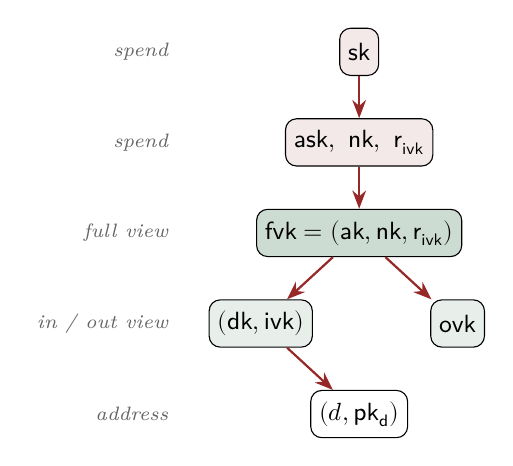
\begin{tikzpicture}[font=\small, x=1cm, y=1cm,
  k/.style={draw, rounded corners, inner sep=3pt, minimum height=6mm,
            anchor=center, fill=arb!10},
  kspend/.style={k, fill=arbred!10},
  kfull/.style={k, fill=arb!22},
  kpub/.style={k, fill=white},
  tier/.style={font=\scriptsize\itshape, text=arbdim, anchor=east},
  op/.style={font=\footnotesize, anchor=west, align=left},
  ow/.style={-{Stealth}, thick, arbred}]
\node[kspend] (sk)  at (0,0)     {$\sksym$};
\node[kspend] (mid) at (0,-1.15) {$\asksym,\ \nksym,\ \rivk$};
\node[kfull]  (fvk) at (0,-2.3)  {$\fvk = (\aksym, \nksym, \rivk)$};
\node[k]      (ivk) at (-1.25,-3.45) {$(\dk, \ivk)$};
\node[k]      (ovk) at (1.25,-3.45)  {$\ovk$};
\node[kpub]   (adr) at (0,-4.6)  {$(d, \pkd)$};
\draw[ow] (sk) -- (mid); \draw[ow] (mid) -- (fvk);
\draw[ow] (fvk) -- (ivk); \draw[ow] (fvk) -- (ovk);
\draw[ow] (ivk) -- (adr);
\node[tier] at (-2.3,0)     {spend};
\node[tier] at (-2.3,-1.15) {spend};
\node[tier] at (-2.3,-2.3)  {full view};
\node[tier] at (-2.3,-3.45) {in / out view};
\node[tier] at (-2.3,-4.6)  {address};
\end{tikzpicture}}

\title{Shielded Zcash}
\subtitle{the Orchard protocol and Halo 2, with the mathematics}
\author{m@rek.onl}
\date{}

\begin{document}

\begin{frame}[plain]
\titlepage
\end{frame}

% ====================================================================
\divider{The problem}

\begin{frame}{What a shielded payment must achieve}
\small
\begin{tabular}{@{}l>{\raggedright\arraybackslash}p{0.39\textwidth}>{\raggedright\arraybackslash}p{0.37\textwidth}@{}}
\toprule
& soundness: every valid payment & hiding: an observer learns \\
\midrule
R1 & the record of a created note binds the note & neither address nor value; real $=$ dummy \\
R2 & a consumed note of value $\neq 0$ was committed at the anchor & not which note \\
R3 & no note is consumed twice & no list of consumed notes \\
R4 & $\sum v\old = \sum v\new + \vb$ & only $\vb$ \\
R5 & only the key holder consumes; data it signs cannot change & --- \\
\bottomrule
\end{tabular}
\vfill
An \emph{observer} reads the chain and holds no key of the notes concerned.
\end{frame}

\begin{frame}{Verification is divided}
\begin{center}
\scalebox{1.2}{\ActionBox}
\end{center}
\small
Per bundle one proof, for one relation per Action, and one binding
signature; per Action one spend-authorisation signature; against chain
state the anchor and the nullifiers.
\end{frame}

% ====================================================================
\divider{Fields, curves, encodings}

\begin{frame}{The Pasta cycle}
\begin{align*}
\pP &= 2^{254} + 45560315531419706090280762371685220353 \\
\pV &= 2^{254} + 45560315531506369815346746415080538113
\end{align*}
\vfill
\begin{center}
\begin{tabular}{@{}lll@{}}
\toprule
curve & equation & group order \\
\midrule
Pallas & $y^2 = x^3 + 5$ over $\FP$ & $|\EP| = \pV$ \\
Vesta & $y^2 = x^3 + 5$ over $\FV$ & $|\Ep(\FV)| = \pP$ \\
\bottomrule
\end{tabular}
\end{center}
\vfill
Both groups have prime order; each curve's scalar field is the other's base
field. Discrete logarithms: about $2^{126}$ group operations.
\types{Pallas points are the protocol's objects; the proof system commits on Vesta, whose scalars are $\FP$.}
\end{frame}

\begin{frame}{Encodings and coordinate extraction}
\small
\[
\LE{k}(m) := b_0 b_1 \cdots b_{k-1}\ \text{ with }\ m = \textstyle\sum_i b_i 2^i
\]
The map $\Ilep{k}$ sends the same integer to $\lceil k/8 \rceil$ little-endian bytes.
\[
\mathcal{O}^{\star} := \LE{256}(0),\qquad
(x, y)^{\star} := \LE{256}\bigl(x + 2^{255} (y \bmod 2)\bigr)
\]
\[
\Ext(\mathcal{O}) := 0,\qquad \Ext\bigl((x, y)\bigr) := x
\]
\vfill
\stmt{Lemma.}{The map $\Ext$ vanishes only at $\mathcal{O}$, since $5$ is a
non-square in $\FP$; and $\Ext(P) = \Ext(P')$ if and only if $P' = \pm P$.}
\vfill
The partial inverse $\mathsf{abst}_{\PP}$ rejects $\tilde x \ge \pP$ and
non-squares $x^3 + 5$: the star encoding is canonical.
\types{$P^{\star} \in \{0,1\}^{256}$; $\Ext \colon \EP \to \FP$.}
\end{frame}

\begin{frame}{Generators from a hash}
\small
The point $\GroupHash(D, M) \in \EP$: $\mathsf{hash\_to\_field}$ by
$\mathsf{expand\_message\_xmd}$ over BLAKE2b-512 gives $u_0, u_1 \in \FP$;
simplified SWU maps each to a curve $3$-isogenous to Pallas; add; apply the
isogeny.
\[
\mathsf{DST} := D \,\|\, \texttt{-pallas\_XMD:BLAKE2b\_SSWU\_RO\_}
\]
\begin{center}
\begin{tabular}{@{}lll@{}}
\toprule
$(D, M)$ & generator & use \\
\midrule
$(\texttt{z.cash:Orchard}, \texttt{G})$ & $\GS$ & spend authorisation \\
$(\texttt{z.cash:Orchard}, \texttt{K})$ & $\KO$ & nullifiers \\
$(\texttt{z.cash:Orchard-cv}, \texttt{v})$, $(\dots, \texttt{r})$ & $\VO, \RO$ & value commitments \\
$(\texttt{z.cash:Orchard-gd}, d)$ & $\gd$ & diversified bases \\
$(\texttt{z.cash:SinsemillaS}, \Ilep{32}(j))$ & $S(j)$ & Sinsemilla table \\
\bottomrule
\end{tabular}
\end{center}
\stmt{Assumption (random oracle).}{Distinct pairs $(D, M)$ receive independent uniform points.}
\end{frame}

% ====================================================================
\divider{Primitives}

\begin{frame}{Expansion and reduction}
\[
\PRFx{k}(t) := \mathrm{BLAKE2b\text{-}512}\bigl(\texttt{Zcash\_ExpandSeed},\ k \,\|\, t\bigr) \in \{0,1\}^{512}
\]
\begin{align*}
\mathrm{ToBase}(x) &:= \mathsf{LEOS2IP}_{512}(x) \bmod \pP \in \FP, \\
\mathrm{ToScalar}(x) &:= \mathsf{LEOS2IP}_{512}(x) \bmod \pV \in \FV
\end{align*}
\vfill
\small
\begin{center}
\begin{tabular}{@{}lll@{}}
\toprule
lead byte & key & derives, in order \\
\midrule
$\mathtt{06}$, $\mathtt{07}$, $\mathtt{08}$ & $\sksym$ & $\asksym$, $\nksym$, $\rivk$ \\
$\mathtt{82}$ & $\LE{256}(\rivk)$ & $\dk \,\|\, \ovk$ \\
$\mathtt{04}$, $\mathtt{09}$, $\mathtt{0B}$ & $\rseed$ & $\esk$, $\psi$, $\rcm$ \\
\bottomrule
\end{tabular}
\end{center}
\vfill
A $512$-bit value reduced modulo a $255$-bit prime is within statistical
distance $m/2^{512} < 2^{-257}$ of uniform.
\stmt{Assumption.}{The map $t \mapsto \PRFx{k}(t)$ is a PRF for uniform $k$; distinct lead bytes give independent outputs.}
\end{frame}

\begin{frame}{The Sinsemilla hash}
Chunk width $k = 10$; table $S(j) := \GroupHash(\texttt{z.cash:SinsemillaS}, \Ilep{32}(j))$, $0 \le j < 2^{10}$;
domain base $Q(D) := \GroupHash(\texttt{z.cash:SinsemillaQ}, D)$.
\[
\mathsf{Acc}_0 := Q(D),\qquad
\mathsf{Acc}_i := (\mathsf{Acc}_{i-1} \dotplus S(m_i)) \dotplus \mathsf{Acc}_{i-1}
\quad (1 \le i \le n)
\]
\[
\SinPt(D, M) := \mathsf{Acc}_n,\qquad
\SinHash(D, M) := \Ext^{\bot}(\mathsf{Acc}_n)
\]
\vfill
\begin{itemize}\itemsep4pt
\item The piece $m_i$ is the $i$-th $10$-bit piece of $M$; at most $c = 253$ pieces, since $2^{253} \le (\pV - 1)/2$.
\item Incomplete addition $\dotplus$ returns $\bot$ when an operand is $\mathcal{O}$ or
  the $x$-coordinates agree.
\item In a circuit each step is one table lookup and two additions.
\end{itemize}
\end{frame}

\begin{frame}{Sinsemilla commitments and the three instances}
\[
\hat M := \SinPt(D \,\|\, \texttt{-M},\, M),\qquad
H_D := \GroupHash(D \,\|\, \texttt{-r},\, \varepsilon)
\]
\begin{gather*}
\SinCom_r(D, M) := \hat M + [r]\,H_D \\
\ShortCom_r(D, M) := \Ext^{\bot}\bigl(\SinCom_r(D, M)\bigr)
\end{gather*}
\types{$r \in \FV$; the commitment is $\bot$ when $\hat M = \bot$.}
\vfill
\begin{center}
\begin{tabular}{@{}llrr@{}}
\toprule
instance & form & message bits & chunks \\
\midrule
$\NoteCommit$ & $\SinCom$ & $1086$ & $109$ \\
$\CommitIvk$ & $\ShortCom$ & $510$ & $51$ \\
$\MCRH$ & $\SinHash$ & $520$ & $52$ \\
\bottomrule
\end{tabular}
\end{center}
\end{frame}

\begin{frame}{What Sinsemilla guarantees}
\stmt{Proposition (collision resistance).}{Under the random-oracle model of
$\GroupHash$ and discrete logarithms on Pallas, no efficient algorithm finds
$M \ne M'$ of the domain's one fixed length $l$ with
$\SinPt(D', M) = \pm \SinPt(D', M') \ne \bot$, nor such a message on which
$\SinPt(D', \cdot) = \bot$. Each such output yields a non-trivial
relation $\sum_i [a_i] P_i = \mathcal{O}$ among $Q(D'), S(0), \dots, S(1023)$.}
\vfill
\stmt{Lemma (hiding and binding).}{(i) If $H_D \ne \mathcal{O}$ and $r$ is
uniform on $\FV$, then $\SinCom_r(D, M)$ is uniform on $\EP$ for every $M$
with $\hat M \ne \bot$. (ii) Two openings, with $M \ne M'$ of one length $l$
and commitments not $\bot$, of one commitment give a discrete-logarithm
relation.}
\proofidea{For (i), the point $[r]\,H_D$ is uniform on a group of prime
order. For (ii), the difference $\hat M - \hat M' = [r' - r]\,H_D$ expands
into the generators. Fixed lengths matter: zero padding makes $M$ and
$M \,\|\, 0$ collide.}
\end{frame}

\begin{frame}{Poseidon and the nullifier PRF}
Poseidon over $\FP$: width $3$, rate $2$, capacity $1$, S-box $x \mapsto x^5$,
$8$ full and $56$ partial rounds; $f \colon \FP^3 \to \FP^3$ the permutation.
\[
\mathsf{PoseidonHash}(x, y) := \pi_1\bigl(f(x, y, 2^{65})\bigr)
\]
\[
\mathsf{PRF}^{\mathsf{nfOrchard}}_{\nksym}(\rho) := \mathsf{PoseidonHash}(\nksym, \rho)
\]
\types{$\nksym, \rho \in \FP$; the capacity element $2^{65}$ encodes the input length $2$.}
\vfill
\stmt{Assumption.}{For uniform $\nksym$, $\rho \mapsto \mathsf{PoseidonHash}(\nksym, \rho)$
is a PRF $\FP \to \FP$.}
\vfill
Its status is cryptanalytic, with no reduction to a standard problem; only
nullifier unlinkability uses it.
\end{frame}

\begin{frame}{RedPallas}
Base $B \ne \mathcal{O}$; hash $\Hs(z) := \mathrm{ToScalar}\bigl(\mathrm{BLAKE2b\text{-}512}(\texttt{Zcash\_RedPallasH}, z)\bigr)$;
$\underline{P} := $ the $32$ bytes of $P^{\star}$.
\vfill
\begin{tabular}{@{}ll@{}}
keys & $x \in \FV$, \quad $X := [x]\,B$ \\[4pt]
sign $M$ & $T \leftarrow \{0,1\}^{640}$,\quad $r := \Hs(T \,\|\, \underline X \,\|\, M)$,\quad $R := [r]\,B$ \\
 & $c := \Hs(\underline R \,\|\, \underline X \,\|\, M)$,\quad $S := r + c\,x$,\quad $\sigma := \underline R \,\|\, \Ilep{256}(S)$ \\[4pt]
verify & $R \ne \bot$,\quad $S < \pV$,\quad $[S]\,B = R + [c]\,X$
\end{tabular}
\vfill
\small
\begin{center}
\begin{tabular}{@{}lll@{}}
\toprule
instance & base $B$ & key re-randomisation \\
\midrule
spend authorisation & $\GS$ & yes: $(x + \alpha,\ X + [\alpha]\,B)$ \\
binding signature & $\RO$ & no \\
\bottomrule
\end{tabular}
\end{center}
\end{frame}

% ====================================================================
\divider{Keys and addresses}

\begin{frame}{The spend-side secrets}
\begin{align*}
\asksym &:= \mathrm{ToScalar}\bigl(\PRFx{\sksym}([\mathtt{06}])\bigr) \in \FV \\
\nksym &:= \mathrm{ToBase}\bigl(\PRFx{\sksym}([\mathtt{07}])\bigr) \in \FP \\
\rivk &:= \mathrm{ToScalar}\bigl(\PRFx{\sksym}([\mathtt{08}])\bigr) \in \FV
\end{align*}
\vfill
\[
\akP := [\asksym]\,\GS \in \EP,\qquad \aksym := \Ext(\akP) \in \FP
\]
\vfill
Sign normalisation: if $[\asksym]\,\GS$ has odd $y$, replace $\asksym$ by
$-\asksym$. The point $\akP$ is recovered from $\aksym$ by the even-$y$ lift.
\types{$\sksym \in \{0,1\}^{256}$ uniform; key generation redraws $\sksym$ if $\asksym = 0$ or $\ivk \in \{0, \bot\}$.}
\end{frame}

\begin{frame}{Viewing keys}
\[
\fvk := (\aksym, \nksym, \rivk)
\]
\begin{align*}
\ivk &:= \CommitIvk_{\rivk}(\aksym, \nksym) = \Ext\bigl(\hat M + [\rivk]\,H_D\bigr), \\
\hat M &:= \SinPt\bigl(D \,\|\, \texttt{-M},\
  \LE{255}(\aksym) \,\|\, \LE{255}(\nksym)\bigr), \\
\dk \,\|\, \ovk &:= \PRFx{\LE{256}(\rivk)}\bigl([\mathtt{82}] \,\|\,
  \Ilep{256}(\aksym) \,\|\, \Ilep{256}(\nksym)\bigr)
\end{align*}
\types{$D := \texttt{z.cash:Orchard-CommitIvk}$; $\ivk \in \{1, \dots, \pP - 1\} \subset \FV$ for an accepted key; $\dk, \ovk$ $32$ bytes each.}
\vfill
\stmt{Lemma.}{For $\rivk$ uniform and independent of $(\aksym, \nksym)$ with
$\hat M \ne \bot$, $\ivk$ is $0$ with probability $1/\pV$ and otherwise
uniform on the $(\pV - 1)/2$ $x$-coordinates of non-identity points.}
\vfill
\stmt{Proposition (binding).}{No efficient algorithm finds
$(\aksym, \nksym, \rivk) \ne (\aksym', \nksym', \rivk')$ with equal
$\CommitIvk \ne \bot$.}
\end{frame}

\begin{frame}{Diversified addresses}
For an index $j \in \{0, \dots, 2^{88} - 1\}$:
\begin{align*}
d &:= \mathsf{FF1\text{-}AES256}_{\dk}\bigl(\LE{88}(j)\bigr) \in \{0,1\}^{88} \\
\gd &:= \DivH(d) := T \text{ if } T \ne \mathcal{O},\ \text{else }
  \GroupHash(\texttt{z.cash:Orchard-gd}, \varepsilon), \\
&\phantom{:=}\ \text{where } T := \GroupHash\bigl(\texttt{z.cash:Orchard-gd},\ d\bigr) \\
\pkd &:= [\ivk]\,\gd
\end{align*}
\vfill
The address is $(d, \pkd)$, with $\pkd \ne \mathcal{O}$. One key has
$2^{88}$ addresses, all with transmission keys under the same $\ivk$.
\vfill
\stmt{Proposition (unlinkability).}{For keys with $\mathsf{use\_qsk} =
\mathsf{false}$, given $\aksym$, $\nksym$ and $\ovk$ of two keys, and
addresses of both, no efficient adversary tells which key a
further address at a fresh index belongs to. \grey{Assumptions: FF1 a PRP,
DDH on Pallas, joint hiding of the viewing keys, PRF expansion.}}
\end{frame}

\begin{frame}{The key ladder}
\begin{columns}[c]
\begin{column}{0.42\textwidth}
\centering
\LadderFig
\end{column}
\begin{column}{0.56\textwidth}
\small
\begin{align*}
&\asksym, \nksym, \rivk \text{ from } \PRFx{\sksym}([\mathtt{06}]), ([\mathtt{07}]), ([\mathtt{08}]) \\[3pt]
&\akP := [\asksym]\,\GS,\quad \aksym := \Ext(\akP) \\[3pt]
&\ivk := \CommitIvk_{\rivk}(\aksym, \nksym) \\
&\dk \,\|\, \ovk := \PRFx{\rivk}([\mathtt{82}] \,\|\, \aksym \,\|\, \nksym) \\[3pt]
&d := \mathsf{FF1}_{\dk}(\LE{88}(j)),\quad \gd := \DivH(d) \\
&\pkd := [\ivk]\,\gd
\end{align*}
\vfill
Every arrow is one-way: each lower key is computed from the one above, and
not conversely.
\end{column}
\end{columns}
\end{frame}

\begin{frame}{What each key can do}
\stmt{Proposition (capability separation).}{For an honestly generated key
with $\mathsf{use\_qsk} = \mathsf{false}$, no efficient algorithm, given only}
\begin{enumerate}\itemsep3pt
\item[(a)] the full viewing key $(\aksym, \nksym, \rivk)$, outputs $\asksym$;
\item[(b)] the incoming viewing key $(\dk, \ivk)$, outputs $\nksym$ or $\asksym$;
\item[(c)] $\ovk$, outputs $\ivk$;
\item[(d)] an address $(d, \pkd)$, outputs $\ivk$.
\end{enumerate}
\vfill
\begin{center}\small
\begin{tabular}{@{}lll@{}}
\toprule
key & computes & cannot \\
\midrule
$\sksym$, $\asksym$ & signatures: spend & --- \\
$\fvk$ & nullifiers: detect spends & sign \\
$(\dk, \ivk)$ & decrypt received notes, derive addresses & detect spends \\
$\ovk$ & recover sent notes & decrypt received ones \\
\bottomrule
\end{tabular}
\end{center}
\end{frame}

% ====================================================================
\divider{Notes and the tree}

\begin{frame}{The note}
\[
n = \bigl((d, \pkd),\ v,\ \rho,\ \psi,\ \rcm\bigr)
\]
\begin{center}
\begin{tabular}{@{}lll@{}}
\toprule
field & type & source \\
\midrule
$(d, \pkd)$ & $\{0,1\}^{88} \times (\EP \setminus \{\mathcal{O}\})$ & the recipient's address \\
$v$ & $\{0, \dots, 2^{64} - 1\}$ zatoshi & the amount; $1\ \mathrm{ZEC} = 10^8$ \\
$\rho$ & $\FP$ & the nullifier consumed in the same Action \\
$\psi$ & $\FP$ & derived from the note seed \\
$\rcm$ & $\FV$ & derived from the note seed \\
\bottomrule
\end{tabular}
\end{center}
\vfill
No note appears on the chain in the clear.
\end{frame}

\begin{frame}{The note commitment}
\[
M(n) := \gd^{\star} \,\|\, \pkd^{\star} \,\|\, \LE{64}(v) \,\|\, \LE{255}(\rho) \,\|\, \LE{255}(\psi)
\quad \text{\grey{($1086$ bits)}}
\]
\[
\cmsym := \NoteCommit_{\rcm}(M(n)) = \hat M + [\rcm]\,H_D,\qquad
\cmx := \Ext^{\bot}(\cmsym)
\]
\types{$\hat M$ under $\texttt{z.cash:Orchard-NoteCommit-M}$; $H_D := \GroupHash(\texttt{z.cash:Orchard-NoteCommit-r}, \varepsilon)$.}
\vfill
\stmt{Proposition.}{(a) Perfect hiding: for $\rcm$ uniform, $\cmsym$ is
uniform on $\EP$ for every note content with $\hat M \ne \bot$. (b) Binding:
no efficient algorithm outputs notes $n \ne n'$ with
$\cmx(n) = \cmx(n') \ne \bot$.}
\proofidea{Part (a) is the Lemma on SinsemillaCommit. For (b), distinct $d$
with equal $\gd$ is a $\GroupHash$ relation; otherwise equal extracted
values mean $\cmsym' = \pm\cmsym$, and either sign gives a relation among
the Sinsemilla generators and $H_D$.}
\end{frame}

\begin{frame}{The note seed}
The sender draws $\rseed \leftarrow \{0,1\}^{256}$; with
$\underline\rho := \Ilep{256}(\rho)$ and lead byte $\mathtt{0x03}$:
\begin{align*}
\esk &:= \mathrm{ToScalar}\bigl(\PRFx{\rseed}([\mathtt{04}] \,\|\, \underline\rho)\bigr) \\
\psi &:= \mathrm{ToBase}\bigl(\PRFx{\rseed}([\mathtt{09}] \,\|\, \underline\rho)\bigr) \\
\rcm &:= \mathrm{ToScalar}\bigl(\PRFx{\rseed}(\mathsf{pre\_rcm})\bigr)
\end{align*}
\[
\mathsf{pre\_rcm} := [\mathtt{0B}] \,\|\, \gd^{\star} \,\|\, \pkd^{\star}
  \,\|\, \Ilep{64}(v) \,\|\, \underline\rho \,\|\, \Ilep{256}(\psi)
  \quad \text{\grey{($137$ bytes)}}
\]
\vfill
Redraw $\rseed$ if $\esk = 0$ or $\cmx = \bot$. One seed fixes the note's
randomness and the encryption key; a recipient can re-derive all three.
\end{frame}

\begin{frame}{The note commitment tree}
Depth $32$; layer $32$ holds the leaves, layer $0$ the root.
\begin{align*}
M^{32}_i &:= \begin{cases} \cmx \text{ appended at position } i & i < n \\
  \mathsf{Uncommitted} = 2 & n \le i < 2^{32} \end{cases} \\
M^h_i &:= \MCRH\bigl(h,\ M^{h+1}_{2i},\ M^{h+1}_{2i+1}\bigr) \qquad (0 \le h < 32)
\end{align*}
\[
\MCRH(l, x, y) := \SinHash\bigl(D,\ \LE{10}(31 - l) \,\|\, \LE{255}(x)
  \,\|\, \LE{255}(y)\bigr)
\]
\types{$D := \texttt{z.cash:Orchard-MerkleCRH}$; an output $\bot$ is replaced by $0$; messages of $520$ bits.}
\vfill
The \emph{anchor} of a block is the root $M^0_0$ of its final treestate.
\stmt{Lemma.}{No point $P$ has $\Ext(P) = 2$, since $2^3 + 5 = 13$ is a
non-square in $\FP$: an unused leaf is the commitment of no note.}
\end{frame}

\begin{frame}{Authentication paths}
\begin{columns}[c]
\begin{column}{0.42\textwidth}
\centering
\TreeFig[path]
\end{column}
\begin{column}{0.56\textwidth}
Write $\mathsf{pos} = \sum_{t < 32} b_t 2^t$, siblings $s_0, \dots, s_{31}$,
and $h_t := \MCRH(31 - t, \cdot, \cdot)$:
\[
a_0 := v,\qquad
a_{t+1} := \begin{cases}
  h_t(a_t, s_t) & b_t = 0 \\
  h_t(s_t, a_t) & b_t = 1
\end{cases}
\]
Valid path to $\mathit{rt}$: $a_{32} = \mathit{rt}$.
\end{column}
\end{columns}
\vfill
Every sibling $s_t$ is a function of the leaves published through the
anchoring block, so the holder computes the path from public data and
never sends $\mathsf{pos}$.
\end{frame}

\begin{frame}{Membership soundness}
\stmt{Proposition.}{Let $\mathit{rt}$ be an anchor whose tree holds $n$
leaves $L_0, \dots, L_{n-1}$. From a valid path to $\mathit{rt}$ with
$v \ne L_{\mathsf{pos}}$ one computes either two distinct $520$-bit
messages with a common $10$-bit prefix and equal $\SinHash$, or a message
on which $\SinHash$ returns $\bot$. Hence no efficient adversary, even one
that chooses the leaves, produces such a path; and if $v = \Ext(P)$ for a
point $P$, then $\mathsf{pos} < n$ and $v$ is the leaf appended at
$\mathsf{pos}$.}
\proofidea{walk the two folds from the leaf upwards; the first level at
which they agree after differing yields the collision, and the level tag
$\LE{10}(t)$ of step $t$ makes the two messages share a prefix.}
\end{frame}

% ====================================================================
\divider{Nullifiers}

\begin{frame}{The nullifier}
\begin{align*}
\DNf_{\nksym}(\rho, \psi, \cmsym) &:= \Ext\bigl([s]\,\KO + \cmsym\bigr), \\
s &:= \bigl(\mathsf{PRF}^{\mathsf{nfOrchard}}_{\nksym}(\rho) + \psi\bigr) \bmod \pP
\end{align*}
\types{$\nksym, \rho, \psi \in \FP$; $\cmsym \in \EP$; $\KO := \GroupHash(\texttt{z.cash:Orchard}, \texttt{K})$.}
\vfill
\begin{itemize}\itemsep5pt
\item Deterministic: one note under one key has one nullifier.
\item Keyed: without $\nksym$ the multiplier $s$ is pseudorandom.
\item Bound to the commitment: $\cmsym$ enters additively.
\end{itemize}
\vfill
\textbf{Chaining.} In every Action, $\rho\new := \nfsym\old$. Accepted
Actions of one pool publish distinct nullifiers (the nullifier-set rule),
so within a pool no two created notes share $\rho$.
\end{frame}

\begin{frame}{Uniqueness and unlinkability}
\stmt{Proposition (uniqueness).}{No efficient adversary, holding every key,
outputs notes with commitments $\cmsym \ne \cmsym'$, not $\bot$, and keys
$\nksym, \nksym'$ with equal nullifiers.}
\proofidea{equal $x$-coordinates give $[s]\,\KO + \cmsym = \pm([s']\,\KO + \cmsym')$;
expanding the commitments gives a relation among $\KO$, $H_D$ and the
Sinsemilla generators.}
\vfill
\stmt{Proposition (unlinkability).}{For a key with $\mathsf{use\_qsk} =
\mathsf{false}$, given $(\dk, \ivk)$ and $\akP$ but not $\nksym$, an adversary that submits $q$ notes with distinct $\rho_i$ cannot
tell $\nfsym_i$ from $\Ext([u_i]\,\KO + \cmsym_i)$ with $u_i$ uniform, up
to $\epsilon_{\mathsf{Pos}} + q\,\delta$ plus key-generation terms, where
$\delta = (\pV - \pP)/\pV < 2^{-167}$.}
\end{frame}

% ====================================================================
\divider{Value}

\begin{frame}{Value commitments}
\begin{align*}
\VO &:= \GroupHash(\texttt{z.cash:Orchard-cv}, \texttt{v}), \\
\RO &:= \GroupHash(\texttt{z.cash:Orchard-cv}, \texttt{r})
\end{align*}
\[
\vnet := v\old - v\new \in \{-2^{64} + 1, \dots, 2^{64} - 1\}
\]
\[
\cvnet := \VC_{\rcv}(\vnet) := [\vnet \bmod \pV]\,\VO + [\rcv]\,\RO
\]
\types{$\rcv \in \FV$ drawn uniformly per Action, from no note; $\cvnet \in \EP$.}
\vfill
\stmt{Lemma.}{(i) Perfect hiding: for uniform $\rcv$, $\cvnet$ is uniform on
$\EP$. (ii) Binding: two openings with $v \not\equiv v' \pmod{\pV}$ give
$\log_{\RO}\VO$.}
\end{frame}

\begin{frame}{The binding signature}
Balancing value $\vb \in \{-2^{63}, \dots, 2^{63} - 1\}$: net value leaving
the pool, public.
\[
\mathsf{bsk} := \sum_{i=1}^{n} \rcv_i,\qquad
\mathsf{bvk} := \sum_{i=1}^{n} \cvnet_i - [\vb]\,\VO
\]
\[
\mathsf{bvk} - [\mathsf{bsk}]\,\RO = \Bigl[\sum_i \vnet_i - \vb\Bigr]\,\VO
\]
\vfill
\stmt{Proposition.}{(i) The key satisfies $\mathsf{bvk} = [\mathsf{bsk}]\,\RO$
if and only if $\sum_i \vnet_i \equiv \vb \pmod{\pV}$. (ii) A party that opens every $\cvnet_i$ and
knows $b$ with $\mathsf{bvk} = [b]\,\RO$, while $D := \sum_i v'_i - \vb
\not\equiv 0$, knows $\log_{\RO}\VO = (b - \sum_i r'_i)\,D^{-1}$.}
\vfill
A RedPallas signature under $\mathsf{bvk}$ on base $\RO$ proves knowledge of
$\mathsf{bsk}$.
\end{frame}

\begin{frame}{Modular balance is integer balance}
\stmt{Lemma.}{Let $n < 2^{16}$, $v\old_i, v\new_i \in \{0, \dots, 2^{64} - 1\}$
and $|\vb| \le \mathsf{MAX\_MONEY}$. If
$\sum_i (v\old_i - v\new_i) \equiv \vb \pmod{\pV}$, the two sides are equal
as integers.}
\vfill
\proofidea{their difference has absolute value at most}
\[
(2^{16} - 1)(2^{64} - 1) + \mathsf{MAX\_MONEY}
= 1\,208\,907\,374\,970\,555\,465\,089\,025 < 2^{80} < \pV .
\]
\vfill
The action count and the range of $\vb$ are consensus rules; the $64$-bit
ranges of $v\old$, $v\new$ are enforced inside the proof.
\end{frame}

% ====================================================================
\divider{Spend authorisation}

\begin{frame}{Randomised validating keys}
Per Action the spender draws $\alpha := \Hs(T)$, $T \leftarrow \{0,1\}^{640}$:
\[
\rsk := \asksym + \alpha,\qquad \rk := \akP + [\alpha]\,\GS = [\rsk]\,\GS
\]
The Action publishes $\rk$ and a signature under $\rsk$ on $\mathsf{SigHash}$;
never $\asksym$, $\alpha$, $\akP$ or $\aksym$.
\vfill
\stmt{Proposition (unlinkability).}{For $\alpha_i$ uniform and independent,
$(\rk_1, \dots, \rk_n)$ is uniform on $\EP^n$ whatever the keys $\akP_i$:
two Actions of one key and of two keys are identically distributed. With
$\alpha_i$ from $\Hs$ the distance is at most
$2n(\delta_{512} + (q_h + n)\,2^{-640})$, $\delta_{512} < 2^{-257}$.}
\end{frame}

\begin{frame}{Unforgeability under re-randomisation}
\small
\stmt{Proposition.}{Let $\akP := [x]\,\GS$ for uniform $x$. An adversary with
$q_h$ hash queries and $q_s$ signing queries $(\alpha, M)$, answered under
$x + \alpha$, outputs $(\rk^{*}, M^{*}, \sigma^{*})$ and $\alpha^{*}$ with
$\rk^{*} = \akP + [\alpha^{*}]\,\GS$. If it forges with probability
$\epsilon$, an algorithm without $x$ outputs $x$ with probability at least}
\[
\frac{(\epsilon - \eta)^2}{Q} - \frac{Q}{\pV} - \frac{q_s (q_h + q_s)}{\pV},
\qquad Q := q_h + q_s + 1,
\]
\[
\eta := Q\,\delta_{512} + q_s (q_h + 2 q_s)\,2^{-640}.
\]
\proofidea{simulate signatures by programming $\mathsf{H}$; fork the
adversary at the challenge query; two forgeries with distinct challenges
give $\rsk^{*}$, and $x = \rsk^{*} - \alpha^{*}$.}
\vfill
\normalsize
With every $\alpha = 0$ this is strong unforgeability of RedPallas.
\end{frame}

% ====================================================================
\divider{The Action statement}

\begin{frame}{Bundle flags}
One flags byte $f = \sum_{i=0}^{7} f_i\, 2^i$ per bundle:
\[
\mathsf{enableSpends} := f_0,\qquad \mathsf{enableOutputs} := f_1
\]
\[
\mathsf{enableCrossAddress} := \begin{cases} f_2 & \text{in the Ironwood pool} \\
0 & \text{in the Orchard pool} \end{cases}
\]
\[
\delta := \mathsf{disableCrossAddress} := 1 - \mathsf{enableCrossAddress}
\]
\vfill
\begin{itemize}\itemsep5pt
\item In $\mathsf{flagsIronwood}$ bits $3$--$7$ are reserved and $0$; in
  $\mathsf{flagsOrchard}$ bits $2$--$7$ are.
\item The \emph{expanded receiver} of an address $(d, \pkd)$ is $(\gd, \pkd)$.
\item With $\delta = 1$ an Action may only create its note at the expanded
  receiver of the note it consumes. Every Orchard-pool Action has
  $\delta = 1$ (ZIP 258), which disables cross-address transfers; no value
  enters that pool, by the separate rule $\mathsf{valueBalanceOrchard} \ge 0$.
\end{itemize}
\end{frame}

\begin{frame}{The relation: inputs and types}
\small
The relation $\Rel_{\mathsf{Action}}$ is the set of pairs $(\mathsf{pub}, \mathsf{aux})$ with
\[
\mathsf{pub} = \bigl(\mathit{rt},\ \cvnet,\ \nfsym\old,\ \rk,\ \cmx,\
  \mathsf{enableSpends},\ \mathsf{enableOutputs},\ \delta\bigr)
\]
\vspace{-6pt}
\begin{align*}
\mathsf{aux} = \bigl(&\mathsf{path}, \mathsf{pos},\ \gd\old, \pkd\old, v\old,
  \rho\old, \psi\old, \rcm\old, \cmsym\old,\ \alpha, \akP, \nksym, \rivk, \\
&\gd\new, \pkd\new, v\new, \psi\new, \rcm\new,\ \rcv,\ \mathsf{c}\bigr)
\end{align*}
\vfill
\begin{tabular}{@{}l@{\hspace{1.2em}}l@{}}
$\mathit{rt}, \nfsym\old, \cmx \in \{0, \dots, \pP - 1\}$ & $\cvnet, \rk, \cmsym\old \in \EP$ \\
$\gd\old, \pkd\old, \gd\new, \pkd\new, \akP \in \EP \setminus \{\mathcal{O}\}$ & $v\old, v\new \in \{0, \dots, 2^{64} - 1\}$ \\
$\rho\old, \psi\old, \psi\new, \nksym \in \FP$ & $\rcm\old, \rcm\new, \rivk, \rcv, \alpha < 2^{255}$ \\
$\mathsf{path} \in \{0, \dots, \pP - 1\}^{32}$, $\mathsf{pos} < 2^{32}$ & $\mathsf{c} \in \{0,1\}^{64}$
\end{tabular}
\vfill
Set $\rho\new := \nfsym\old$; $M\old$, $M\new$ are the $1086$-bit note messages.
\end{frame}

\begin{frame}{Conditions A1 to A5}
\small
\begin{description}[A5.]\itemsep6pt
\item[A1.] $\NoteCommit_{\rcm\old}(M\old) \in \{\cmsym\old, \bot\}$
  \rtag{old note commitment integrity}
\item[A2.] $\Ext^{\bot}\bigl(\NoteCommit_{\rcm\new}(M\new)\bigr) \in \{\cmx, \bot\}$
  \rtag{new note commitment integrity}
\item[A3.] $v\old \cdot (\mathit{root} - \mathit{rt}) = 0$, or a hash in the fold returns $\bot$
  \rtag{Merkle path validity}\\
  $\mathit{root} := a_{32}$, the fold from $a_0 := \Ext(\cmsym\old)$ along $(\mathsf{pos}, \mathsf{path})$
\item[A4.] $\cvnet = [v\old - v\new]\,\VO + [\rcv]\,\RO$
  \rtag{value commitment integrity}
\item[A5.] $\nfsym\old = \Ext\bigl([(\mathsf{PRF}^{\mathsf{nfOrchard}}_{\nksym}(\rho\old) + \psi\old) \bmod \pP]\,\KO + \cmsym\old\bigr)$\\
  \rtag{nullifier integrity}
\end{description}
\vfill
The bits $\mathsf{c}$ admit the non-canonical encodings $x + \pP < 2^{255}$
of the fold's arguments; the values $\bot$ cannot be produced efficiently.
\end{frame}

\begin{frame}{Conditions A6 to A10}
\small
\begin{description}[A10.]\itemsep6pt
\item[A6.] $\rk = \akP + [\alpha]\,\GS$ \rtag{spend authority}
\item[A7.] $\ivk := \CommitIvk_{\rivk}(\Ext(\akP), \nksym)$; \ $\ivk = \bot$ or
  $\pkd\old = [\ivk]\,\gd\old$\\ \rtag{diversified address integrity}
\item[A8.] $v\old \cdot (1 - \mathsf{enableSpends}) = 0$ \rtag{enable spends}
\item[A9.] $v\new \cdot (1 - \mathsf{enableOutputs}) = 0$ \rtag{enable outputs}
\item[A10.] $\delta\,(x(\gd\old) - x(\gd\new)) = \delta\,(y(\gd\old) - y(\gd\new)) = 0$,\\
  $\delta\,(x(\pkd\old) - x(\pkd\new)) = \delta\,(y(\pkd\old) - y(\pkd\new)) = 0$
  \rtag{cross-address restriction}
\end{description}
\vfill
Every condition is an equation over $\FP$ or $\EP$: exactly the shape a
circuit over $\FP$ checks.
\end{frame}

\begin{frame}{What the statement enforces, and what is checked outside}
\small
\begin{tabular}{@{}lll@{}}
\toprule
requirement & inside the proof & outside the proof \\
\midrule
R1 hidden value & A1, A2 & --- \\
R2 membership & A1, A3 & the anchor is a past root \\
R3 no double spend & A5, chaining $\rho\new = \nfsym\old$ & $\nfsym$ not in the set \\
R4 conservation & A4, the $64$-bit ranges & binding signature under $\mathsf{bvk}$ \\
R5 authority & A6, A7 & signature under $\rk$ on $\mathsf{SigHash}$ \\
flags, seal & A8, A9, A10 & flags read from the bundle \\
\bottomrule
\end{tabular}
\vfill
Not checked by the statement: the derivation of $\rcm$ and $\psi$ from
$\rseed$, and the note ciphertexts. The recipient checks those.
\end{frame}

\begin{frame}{The proof system, as assumptions}
\stmt{Assumption (knowledge soundness).}{With the Fiat--Shamir hash a random
oracle, for every efficient prover that outputs primary inputs
$\mathsf{pub}_1, \dots, \mathsf{pub}_n$ and an accepted proof there is an
efficient extractor outputting $\mathsf{aux}_1, \dots, \mathsf{aux}_n$
with $(\mathsf{pub}_i, \mathsf{aux}_i) \in \Rel_{\mathsf{Action}}$ for all
$i$, except with negligible probability.}
\vfill
\stmt{Assumption (zero knowledge).}{With a programmable random oracle, a
simulator given only $\mathsf{pub}_1, \dots, \mathsf{pub}_n$ outputs proofs
statistically indistinguishable from honest ones.}
\vfill
One proof per bundle, over $n$ instances of one circuit; the last part of
this deck shows how Halo 2 supports both.
\end{frame}

% ====================================================================
\divider{Note encryption}

\begin{frame}{The note plaintext}
\[
\mathsf{np} := \mathsf{leadByte} \,\|\, d \,\|\, \Ilep{64}(v) \,\|\, \rseed \,\|\, \mathsf{memo}
\]
\begin{center}
\begin{tabular}{@{}lrl@{}}
\toprule
field & bytes & \\
\midrule
$\mathsf{leadByte}$ & $1$ & $\mathtt{0x03}$ in the Ironwood pool \\
$d$ & $11$ & the diversifier \\
$v$ & $8$ & the value \\
$\rseed$ & $32$ & the note seed \\
$\mathsf{memo}$ & $512$ & chosen by the sender \\
\midrule
total & $564$ & fixed: the length reveals nothing \\
\bottomrule
\end{tabular}
\end{center}
\vfill
From $(d, v, \rseed)$ and the Action's $\nfsym\old$ the recipient recomputes
$\gd$, $\psi$, $\rcm$ and $\esk$.
\end{frame}

\begin{frame}{Encryption to the recipient}
\begin{align*}
\epk &:= [\esk]\,\gd,\qquad s := [\esk]\,\pkd \\
K_{\mathrm{enc}} &:= \mathrm{BLAKE2b\text{-}256}\bigl(\texttt{Zcash\_OrchardKDF},\ s^{\star} \,\|\, \epk^{\star}\bigr) \\
\Ecenc &:= \mathrm{ChaCha20\text{-}Poly1305}_{K_{\mathrm{enc}}}(\mathsf{np})
  \quad \text{\grey{(zero nonce, $564 + 16 = 580$ bytes)}}
\end{align*}
\vfill
\stmt{Proposition (correctness).}{If $\pkd = [\ivk]\,\gd$ then
$[\ivk]\,\epk = [\esk]\,\pkd = s$: the holder of $\ivk$ derives the same key.}
\vfill
\stmt{Proposition (confidentiality and key privacy).}{For an honestly
generated recipient with $\mathsf{use\_qsk} = \mathsf{false}$, $(\epk^{\star}, \Ecenc, \cmx)$ is computationally
indistinguishable from a uniform non-identity point, an encryption of a
fixed string under an independent key, and $\cmx$. \grey{DDH on Pallas,
KDF a random oracle, the AEAD, joint hiding of the viewing keys.}}
\end{frame}

\begin{frame}{The outgoing ciphertext}
\begin{align*}
\mathsf{ock} &:= \mathrm{BLAKE2b\text{-}256}\bigl(\texttt{Zcash\_Orchardock},\
  \ovk \,\|\, (\cvnet)^{\star} \,\|\, \Ilep{256}(\cmx) \,\|\, \epk^{\star}\bigr) \\
\mathsf{op} &:= \pkd^{\star} \,\|\, \Ilep{256}(\esk) \quad \text{\grey{($64$ bytes)}} \\
\Ecout &:= \mathrm{ChaCha20\text{-}Poly1305}_{\mathsf{ock}}(\mathsf{op})
  \quad \text{\grey{($80$ bytes)}}
\end{align*}
\vfill
The sender's $\ovk$ recovers $(\pkd, \esk)$, hence $s = [\esk]\,\pkd$ and
the note: a wallet reconstructs what it sent. With $\ovk = \bot$ both
$\mathsf{ock}$ and $\mathsf{op}$ are random and nothing is recoverable.
\end{frame}

\begin{frame}{Trial decryption and acceptance}
For every Action: $s := [\ivk]\,\epk$, $K_{\mathrm{enc}} := \mathsf{KDF}(s, \epk)$,
$\mathsf{np} := \mathrm{Dec}_{K_{\mathrm{enc}}}(\Ecenc)$; a result $\ne \bot$
is a candidate. For an Ironwood-pool output, accept only if:
\begin{enumerate}\itemsep4pt
\item[(i)] $\mathsf{leadByte} = \mathtt{0x03}$;
\item[(ii)] with $\rho := \nfsym\old$: $\gd := \DivH(d)$, $\pkd := [\ivk]\,\gd$,
  then $\psi$, then $\rcm$ from $\rseed$;
\item[(iii)] $([\esk]\,\gd)^{\star} = \epk^{\star}$ for $\esk$ from $\rseed$;
\item[(iv)] $\Ext\bigl(\NoteCommit_{\rcm}(M(n))\bigr) = \cmx$.
\end{enumerate}
\vfill
\stmt{Proposition.}{An accepted note is addressed to the recipient's key,
carries $\rho = \nfsym\old$, and is the unique opening of $\cmx$: no sender
can make the recipient accept $n$ while holding $n' \ne n$ with
$\cmx(n') = \cmx$.}
\end{frame}

% ====================================================================
\divider{Transactions and consensus}

\begin{frame}{The Action description}
\begin{center}
\begin{tabular}{@{}lrl@{}}
\toprule
field & bytes & \\
\midrule
$(\cvnet)^{\star}$ & $32$ & net value commitment \\
$\Ilep{256}(\nfsym)$ & $32$ & nullifier of the consumed note \\
$\rk^{\star}$ & $32$ & randomised validating key \\
$\Ilep{256}(\cmx)$ & $32$ & extracted commitment of the created note \\
$\epk^{\star}$ & $32$ & ephemeral public key \\
$\Ecenc$ & $580$ & note ciphertext \\
$\Ecout$ & $80$ & outgoing ciphertext \\
\midrule
& $820$ & \\
\bottomrule
\end{tabular}
\end{center}
\vfill
Per bundle: flags ($1$), $\vb$ ($8$), anchor ($32$), proof
($2720 + 2272\,n$), $n$ spend signatures and one binding signature ($64$ each).
\end{frame}

\begin{frame}{Digests: what the signatures sign}
\small
\[
\mathsf{txid} := \mathsf{h}\bigl(\texttt{ZcashTxHash\_} \,\|\, \beta,\
  d_{\mathsf{hdr}} \,\|\, d_{\mathsf{tr}} \,\|\, d_{\mathsf{Sap}}
  \,\|\, d_{\mathsf{Orc}} \,\|\, d_{\mathsf{Irw}}\bigr)
\]
\[
d_{\mathsf{Irw}} := \mathsf{h}\bigl(\texttt{ZTxIdIronwd\_H\_v6},\
  d_{\mathsf{C}} \,\|\, d_{\mathsf{M}} \,\|\, d_{\mathsf{N}} \,\|\,
  \mathsf{flags} \,\|\, \vb\bigr)
\]
\types{The hash $\mathsf{h}$ is BLAKE2b-256 under a $16$-byte personalisation; $\beta$ the consensus branch identifier; $d_{\mathsf{C}}, d_{\mathsf{M}}, d_{\mathsf{N}}$ hash the Actions' compact, memo and remaining fields.}
\vfill
For a transaction without transparent inputs the signature digest
$\mathsf{SigHash}$ equals $\mathsf{txid}$; otherwise its transparent child
also commits to the spent coins' values and scripts. It is the message of
every spend-authorisation signature and of each binding signature.
\vfill
\stmt{Proposition (bundle binding).}{Under collision resistance of
BLAKE2b, discrete logarithms on Pallas and $\mathsf{H}$ a random oracle, no
efficient adversary, against honestly generated keys whose holders sign
only $\mathsf{SigHash}(T)$ under each $\rk$, produces an accepted
transaction that reuses an Action's $\rk$ and changes the effecting data,
except with negligible probability. The anchor and the proof are not signed:
they are authorising data, and the proof binds the anchor.}
\end{frame}

\begin{frame}{Verification}
\small
A version-$6$ transaction is accepted, for its Orchard-protocol bundles, iff:
\begin{enumerate}\itemsep3pt
\item every field parses canonically; counts, reserved bits, flags, ranges;
\item the proof verifies on the $n$ primary inputs
  $(\mathit{rt}, \cvnet_i, \nfsym_i, \rk_i, \cmx_i, f_0, f_1, \delta)$
  \rtag{R1--R5 via A1--A10}
\item $\mathit{rt}$ is the root of the pool's tree at an earlier block
  \rtag{R2}
\item no nullifier repeats, in the transaction or the pool's set
  \rtag{R3}
\item each spend signature verifies under $\rk_i$ on $\mathsf{SigHash}$
  \rtag{R5}
\item the binding signature verifies under $\mathsf{bvk}$; the fee is
  $\ge 0$ \rtag{R4}
\item pool rules: expiry, tree capacity, chain value pool balances.
\end{enumerate}
\vfill
On acceptance: nullifiers enter the pool's set, each $\cmx$ is appended to
its tree, and the pool's balance decreases by $\vb$.
\end{frame}

\begin{frame}{As specified for NU7}
\begin{itemize}\itemsep6pt
\item Block target spacing $25$\,s (ZIP 218); the default expiry delta is
  $120$ blocks, $3000$\,s $= 50$ minutes; an anchor depth of $3$ blocks is
  $75$\,s.
\item Version-$4$ transactions are invalid (ZIP 2003); versions $5$ and $6$
  remain, with no new format (ZIP 259).
\item Per-block shielded limits (ZIP 218): $\mathsf{OrchardBlockActionLimit}
  = \mathsf{GlobalShieldedBudget} = 330$, as written counting
  Orchard-pool Actions only.
\item The Orchard pool stays sealed, as from NU6.3 (ZIP 258): no
  Orchard-pool Actions in coinbase, $\delta = 1$ in every Orchard-pool
  Action, and $\mathsf{valueBalanceOrchard} \ge 0$.
\end{itemize}
\vfill
ZIP 259, which deploys NU7, has status Draft.
\end{frame}

\begin{frame}{A worked payment}
\small
Alice holds a note of $7$ ZEC in the Ironwood pool and pays Bob $5$ ZEC.
\begin{center}
\begin{tabular}{@{}lrrr@{}}
\toprule
Action & $v\old$ & $v\new$ & $\vnet$ \\
\midrule
1: Alice's note $\to$ Bob & $700\,000\,000$ & $500\,000\,000$ & $200\,000\,000$ \\
2: dummy $\to$ Alice's change & $0$ & $199\,990\,000$ & $-199\,990\,000$ \\
\midrule
$\vb = \sum \vnet$ & & & $10\,000$ \\
\bottomrule
\end{tabular}
\end{center}
\begin{itemize}\itemsep3pt
\item Fee $5000 \cdot \max(2, 2) = 10\,000$ zatoshi (ZIP 317), paid by $\vb > 0$
  into the transparent value pool.
\item The binding key is $\mathsf{bvk} = \sum \cvnet_i - [10\,000]\,\VO = [\rcv_1 + \rcv_2]\,\RO$.
\item The flag $\mathsf{enableCrossAddress}$ is $1$: Action 1 pays a receiver other than
  its consumed note's.
\item The Ironwood component: $9141$ bytes, of which the proof $7264$.
\end{itemize}
\end{frame}

% ====================================================================
\divider{Security}

\begin{frame}{Assumptions, listed once}
\small
\begin{tabular}{@{}ll@{}}
\toprule
assumption & used for \\
\midrule
discrete logarithms on Pallas & every binding and uniqueness result \\
$\GroupHash$ a random oracle & independent generators \\
knowledge soundness of the Action proof & every soundness theorem \\
zero knowledge of the Action proof & privacy \\
$\mathsf{PRFexpand}$ a PRF & keys, note seeds \\
Poseidon a PRF & nullifier unlinkability \\
DDH on Pallas; FF1 a PRP & note encryption; address unlinkability \\
joint hiding of the viewing keys & capabilities, privacy \\
$\mathsf{H}$, $\mathsf{KDF}$, $\mathsf{PRF}^{\mathsf{ock}}$ random oracles & signatures, encryption \\
ChaCha20-Poly1305 IND-CPA, INT-CTXT & note encryption \\
BLAKE2b collision resistance & bundle binding \\
\bottomrule
\end{tabular}
\vfill
Each theorem names the ones it uses; none is a theorem itself.
\end{frame}

\begin{frame}{Balance}
\stmt{Theorem.}{For each pool, every accepted bundle output by an efficient
adversary satisfies $\sum_{i=1}^{n} (v\old_i - v\new_i) = \vb$ as integers,
the values read from the extracted witnesses, except with negligible
probability.}
\proofidea{Extract the witnesses (knowledge soundness). By A4 each $\cvnet_i$
opens to $(v\old_i - v\new_i, \rcv_i)$. The binding signature verifies under
$\mathsf{bvk}$, so a key $b$ with $\mathsf{bvk} = [b]\,\RO$ is extracted by
forking. If $\sum_i \vnet_i \not\equiv \vb$, part (ii) of the binding
proposition gives $\log_{\RO}\VO$, a discrete-logarithm relation between two
$\GroupHash$ outputs. So the sum holds modulo $\pV$, hence over the integers
by the $2^{80}$ bound.}
\end{frame}

\begin{frame}{No double-spending}
\stmt{Lemma.}{Two accepted Actions whose witnessed consumed notes have the
same $\Ext(\cmsym\old)$ consume the same note under the same $\nksym$ and
publish the same $\nfsym\old$.}
\proofidea{Condition A1 and binding of $\NoteCommit$ fix the note, hence $(\gd\old,
\pkd\old)$; by A7, $\pkd\old = [\ivk]\,\gd\old$ fixes $\ivk$, and binding
of $\CommitIvk$ fixes $(\aksym, \nksym)$; A5 is then determined.}
\vfill
\stmt{Theorem.}{For each pool, no committed note of non-zero value is
consumed by two accepted Actions of that pool, except with negligible
probability.}
\proofidea{Membership (A3) makes each consumed note a leaf; the lemma gives
one nullifier; the nullifier rule rejects the second.}
\vfill
\stmt{Corollary (Faerie Gold).}{Distinct accepted Actions of one pool
create notes with distinct $\rho$; distinct notes have distinct nullifiers.}
\end{frame}

\begin{frame}{Spend authority}
\stmt{Experiment.}{The adversary gets the full viewing key $(\aksym, \nksym,
\rivk)$, not $\asksym$, and signatures on queries $(\alpha, m)$ under
$\asksym + \alpha$. It wins with an accepted Action that consumes a note of
the key and carries a valid signature under its $\rk$ on some $m$ with no
query $(\alpha, m)$ satisfying $\rk = \akP + [\alpha]\,\GS$.}
\vfill
\stmt{Theorem.}{No efficient adversary wins, except with negligible
probability. \grey{Keys with $\mathsf{use\_qsk} = \mathsf{false}$.}}
\proofidea{Extract the witness: by A7 and binding of $\CommitIvk$ its point
is $\pm$ the key's $\akP$, and A6 gives $\rk = \pm\akP + [\alpha]\,\GS$.
The signature is then a forgery under re-randomisation, from which forking
extracts $\rsk^{*}$ and hence $\asksym = \pm(\rsk^{*} - \alpha)$: a discrete
logarithm of $\akP$.}
\end{frame}

\begin{frame}{Privacy}
\small
\stmt{Theorem.}{Under preconditions (honest keys, construction as specified,
local paths, no viewing key of a party held), two Ironwood-pool bundles with
equal public leakage (pool, number of Actions, anchor, flags, $\vb$) have
computationally indistinguishable public data. In particular a dummy
Action is indistinguishable from a real one.}
\vfill
\proofidea{a sequence of hybrids, each justified by one assumption:}
\begin{center}
\begin{tabular}{@{}ll@{}}
\toprule
replace & justified by \\
\midrule
the proof by a simulated one & zero knowledge \\
$\cvnet$, $\rk$ by uniform points & perfect hiding; uniform $\alpha$ \\
$\nfsym$ by $\Ext([u]\,\KO + \cmsym)$ & Poseidon PRF, joint hiding \\
$\Ecout$ by an encryption of a fixed string & $\mathsf{PRF}^{\mathsf{ock}}$ oracle, AEAD \\
$\epk^{\star}, \Ecenc$ by random ones & DDH, KDF oracle, AEAD \\
$\cmx$ by $\Ext$ of a uniform point & PRF expansion, then perfect hiding \\
\bottomrule
\end{tabular}
\end{center}
\end{frame}

\begin{frame}{The end-to-end theorem}
\small
For each pool, no efficient adversary achieves any of the following, except
with negligible probability:
\begin{enumerate}\itemsep4pt
\item[(i)] an accepted Action with no extractable witness, a second opening
  of a created $\cmx$, or a consumed note of non-zero value that is not a
  leaf at the anchor \rtag{R1, R2}
\item[(ii)] two accepted Actions consuming one committed note of non-zero
  value \rtag{R3}
\item[(iii)] an accepted bundle whose $\vb$ differs from
  $\sum (v\old - v\new)$ \rtag{R4}
\item[(iv)] consuming a note of an honest key without its holder's
  signature, or changing the signed data of a transaction \rtag{R5}
\item[(v)] for the Ironwood pool, distinguishing two bundles with equal
  public leakage \rtag{hiding of R1--R4}
\end{enumerate}
\vfill
\normalsize
Clauses (i)--(iii) use no property of key generation; (iv) and (v) are
claimed for keys with $\mathsf{use\_qsk} = \mathsf{false}$.
\end{frame}

% ====================================================================
\divider{How Halo 2 proves}

\begin{frame}{PLONKish constraint systems}
\small
Over a prime field $\F$, with $n = 2^k$ rows labelled by
$H := \{\omega^0, \dots, \omega^{n-1}\}$, $\ZH(X) := X^n - 1$:
\begin{enumerate}\itemsep4pt
\item columns of $n$ cells: \emph{fixed} (the circuit), \emph{advice} (the
  witness), \emph{instance} (public inputs);
\item custom gates $g_t = 0$ of degree $\le d_{\max}$ in cells of the current
  row and of rows at fixed \emph{rotations} $v(\omega^r X)$;
\item equality constraints: a permutation $\sigma$ of a set of cells whose
  cycles must hold equal values;
\item lookups: input expressions $(A_0, \dots, A_{m-1})$ whose every row is a
  row of a table $(S_0, \dots, S_{m-1})$.
\end{enumerate}
\vfill
A column is its interpolant: $v(X)$ of degree $< n$ with $v(\omega^i) =$ the
cell of row $i$. A constraint holds on every row iff its polynomial is
divisible by $\ZH$.
\end{frame}

\begin{frame}{The toy: a table}
``I know $x$ with $x^3 + x + 5 = 35$'' over $\F_{97}$; the witness $x = 3$.
\[
q_M\, a\, b + q_L\, a + q_R\, b + q_O\, c + q_C + \mathrm{PI} = 0
\quad\text{on every row}
\]
\begin{center}\small
\begin{tabular}{@{}c ccc ccccc c l@{}}
\toprule
& \multicolumn{3}{c}{advice} & \multicolumn{5}{c}{fixed} & instance & \\
\cmidrule(lr){2-4}\cmidrule(lr){5-9}\cmidrule(lr){10-10}
row & $a$ & $b$ & $c$ & $q_M$ & $q_L$ & $q_R$ & $q_O$ & $q_C$
  & $\mathrm{PI}$ & \\
\midrule
0 & 3 & 3 & 9 & 1 & 0 & 0 & $-1$ & 0 & 0 & $x \cdot x = x^2$ \\
1 & 9 & 3 & 27 & 1 & 0 & 0 & $-1$ & 0 & 0 & $x^2 \cdot x = x^3$ \\
2 & 27 & 3 & 30 & 0 & 1 & 1 & $-1$ & 0 & 0 & $x^3 + x = s$ \\
3 & 30 & 0 & 0 & 0 & 1 & 0 & 0 & 5 & $-35$ & $s + 5 = 35$ \\
\bottomrule
\end{tabular}
\end{center}
Copy constraints: $a_0 = b_0 = b_1 = b_2 = x$; $c_i = a_{i+1}$.
\end{frame}

\begin{frame}{Rows become polynomials}
The element $\omega = 22$ has order $4$ in $\F_{97}$: $H = \{1, 22, 96, 75\}$, $\ZH(X) = X^4 - 1$.
\[
a(1) = 3,\ a(22) = 9,\ a(96) = 27,\ a(75) = 30
\ \Longrightarrow\
a(X) = 90 + 61X + 22X^2 + 24X^3
\]
\[
G(X) := q_M a b + q_L a + q_R b + q_O c + q_C + \mathrm{PI},\qquad \deg G \le 9
\]
\vfill
\stmt{Theorem.}{Every gate holds $\iff$ $G$ vanishes on $H$ $\iff$ $\ZH \mid
G$ $\iff$ $G = t \cdot \ZH$ for some polynomial $t$.}
\vfill
The lie $x^2 = 10$ in row $0$ leaves, for any $t^{*}$, a nonzero gap
$D := G^{*} - t^{*}\ZH$; for the Euclidean quotient $D = 24\,(1 + X + X^2 + X^3)$.
\end{frame}

\begin{frame}{One random point}
\stmt{Theorem (Schwartz--Zippel).}{If the trace is invalid and the committed
$G^{*}, t^{*}$ are fixed before $z$ is drawn uniformly from $\F$, then}
\[
\Pr_z\bigl[G^{*}(z) = t^{*}(z)\,\ZH(z)\bigr] = \Pr_z[D(z) = 0] \le \frac{\deg D}{|\F|}.
\]
\begin{center}
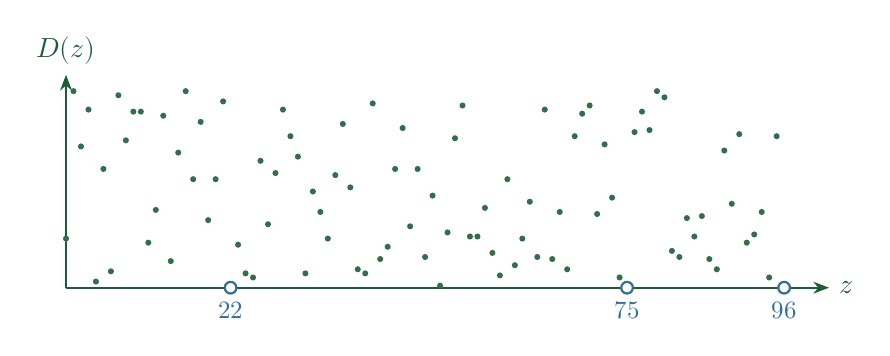
\begin{tikzpicture}[x=.095cm,y=.026cm]
\draw[flow] (0,0)--(102,0) node[right] {$z$};
\draw[flow] (0,0)--(0,104) node[above] {$D(z)$};
\foreach \x in {0,...,96}{
  \pgfmathtruncatemacro{\square}{mod(\x*\x,97)}
  \pgfmathtruncatemacro{\cube}{mod(\square*\x,97)}
  \pgfmathtruncatemacro{\residue}{mod(24*(1+\x+\square+\cube),97)}
  \fill[arb!90] (\x,\residue) circle[radius=1.1pt];
}
\foreach \x in {22,75,96}{
  \draw[tierin!85!black,thick,fill=white] (\x,0) circle[radius=2.1pt];
  \node[below,font=\small,text=tierin!85!black] at (\x,-2) {$\x$};
}
\end{tikzpicture}
\end{center}
Toy: $3/97$. Deployed: $\deg D < 9 \cdot 2^{11}$, so $\le 18432/\pP < 2^{-239}$.
\end{frame}

\begin{frame}{The permutation argument}
\small
Cells $(i, j)$ of the $m$ equality columns get labels $\delta^i \omega^j$;
fixed polynomials $s_i$ hold the labels permuted by $\sigma$. After
challenges $\beta, \gamma$ the prover commits to $Z_{\mathrm{perm}}$ with
\begin{align*}
\ell_0(X)\,\bigl(1 - Z_{\mathrm{perm}}(X)\bigr) &\equiv 0 \\
Z_{\mathrm{perm}}(\omega X) \prod_i \bigl(v_i + \beta s_i + \gamma\bigr)
- Z_{\mathrm{perm}}(X) \prod_i \bigl(v_i + \beta \delta^i X + \gamma\bigr) &\equiv 0
\end{align*}
modulo $\ZH$: together
\[
\prod_{i,j} \bigl(v_i(\omega^j) + \beta\,\delta^i \omega^j + \gamma\bigr)
= \prod_{i,j} \bigl(v_i(\omega^j) + \beta\,s_i(\omega^j) + \gamma\bigr).
\]
\stmt{Theorem.}{The copy constraints hold iff the two products agree as
polynomials in $(\beta, \gamma)$; a violation survives random $\beta, \gamma$
with probability $\le 2N/|\F|$, $N$ the number of cells.}
\end{frame}

\begin{frame}{The lookup argument}
\small
Goal: every value of $A$ on the active rows occurs in $S$. The prover
commits to $A'$, a permutation of $A$ with equal values in runs, and $S'$,
a permutation of $S$ with each run's value at its first row; after
$\beta, \gamma$, to $Z_{\mathrm{lookup}}$:
\begin{align*}
\ell_0(X)\,\bigl(1 - Z_{\mathrm{lookup}}(X)\bigr) &\equiv 0 \\
Z_{\mathrm{lookup}}(\omega X)\,(A' + \beta)(S' + \gamma)
  - Z_{\mathrm{lookup}}(X)\,(A + \beta)(S + \gamma) &\equiv 0 \\
\ell_0(X)\,(A' - S') &\equiv 0 \\
(A' - S')\,\bigl(A'(X) - A'(\omega^{-1} X)\bigr) &\equiv 0
\end{align*}
modulo $\ZH$ on the active rows.
\vfill
\stmt{Theorem.}{If the identities hold, then except with probability
$\le 4n/|\F|$ every value of $A$ on the active rows is a value of $S$.}
\types{Toy: $S = (0,1,2,3)$, $A = (2,3,2,2)$, $A' = (2,2,2,3)$, $S' = (2,0,1,3)$.}
\end{frame}

\begin{frame}{The vanishing argument}
All constraints $g_0, \dots, g_{m-1}$ (gates, permutation rules, lookup rules)
are combined with a challenge $y$:
\[
h(X) := \frac{\sum_{i} y^i\, g_i(X)}{\ZH(X)},\qquad
h(X) = \sum_{j=0}^{d_{\max}-2} X^{nj}\, h_j(X)
\]
\types{each $h_j$ of degree $< n$ is committed separately.}
\vfill
\stmt{Theorem.}{The quotient satisfies $\deg h \le d_{\max}(n - 1) - n = (d_{\max} - 1)(n - 1) - 1$.}
\vfill
At a challenge $x$ the prover sends the value at $x$ and at the needed
rotations $\omega^r x$ of every committed polynomial except the pieces
$h_j$. The verifier computes $\sum_i y^i g_i(x) / \ZH(x)$, and the opening
argument checks it against $\sum_j [x^{nj}]\,\mathsf{Comm}(h_j)$.
\types{Action circuit: $d_{\max} = 9$, $n = 2^{11}$, so $\deg h \le 16375$.}
\end{frame}

\begin{frame}{The transcript, and Fiat--Shamir}
\begin{center}\small
\begin{tabular}{@{}ll@{}}
\toprule
prover sends & then the challenge \\
\midrule
commitments to the advice columns & $\theta$ \\
permuted lookup columns $A', S'$ & $\beta, \gamma$ \\
permutation and lookup products $Z$; a random polynomial & $y$ \\
the pieces $h_j$ of the quotient & $x$ \\
all evaluations at $x$ and $\omega^r x$ & $x_1, x_2$ \\
the multipoint quotient commitment & $x_3$ \\
the values $q_i(x_3)$ & $x_4$ \\
the mask commitment $S$ & $\xi, \zeta$ \\
$(L_j, R_j)$, one pair per round & $u_j$ \\
\bottomrule
\end{tabular}
\end{center}
\vfill
Each challenge is a hash of the transcript so far: the verifier's coins
become a function of everything the prover has committed to.
\end{frame}

\begin{frame}{Many openings to one}
\small
Polynomials $p_\nu$ with commitments $C_\nu$, grouped by their query sets
$T^{(i)}$, $Z_i(X) := \prod_{t \in T^{(i)}} (X - t)$:
\begin{enumerate}\itemsep3pt
\item Challenge $x_1$: \ $q_i := \sum_e x_1^e\, p_{\nu_{i,e}}$, \ $Q_i := \sum_e [x_1^e]\,C_{\nu_{i,e}}$; \ $r_i$ interpolates the claimed values on $T^{(i)}$;
\item Challenge $x_2$: \ $f := \sum_i x_2^{i-1} (q_i - r_i)/Z_i$, committed as $F$;
\item Challenge $x_3$: \ the prover sends $u_i := q_i(x_3)$; the verifier forms
  $v_f := \sum_i x_2^{i-1} \dfrac{u_i - r_i(x_3)}{Z_i(x_3)}$;
\item Challenge $x_4$: \ $f^{*} := f + \sum_i x_4^i q_i$, \ $F^{*} := F + \sum_i [x_4^i]\,Q_i$,
  \ $v^{*} := v_f + \sum_i x_4^i u_i$.
\end{enumerate}
\vfill
One opening of $F^{*}$ at $x_3$ to $v^{*}$ replaces them all: $f$ is a
polynomial only if every claimed value is true.
\end{frame}

\begin{frame}{The inner-product commitment}
Generators $\bfG = (G_0, \dots, G_{d-1})$, $H$, $U$ on Vesta, from a hash;
$d = 2^k$.
\[
\mathsf{Comm}(p; r) := \langle \bfa, \bfG \rangle + [r]\,H,\qquad
p(X) = \sum_{i < d} a_i X^i
\]
\[
\Rel_{\mathrm{IPA}} := \bigl\{ \bigl((P, x, v);\, (\bfa, r)\bigr) :
  P = \langle \bfa, \bfG \rangle + [r]\,H,\ v = \langle \bfa, \bfb(x) \rangle \bigr\}
\]
\[
\bfb(x) := (1, x, \dots, x^{d-1})
\]
\types{$a_i, r, x, v \in \FP$, the scalar field of Vesta; $P, \bfG, H, U \in \Ep(\FV)$.}
\vfill
Pedersen on the coefficient vector: perfectly hiding, binding under
discrete logarithms on Vesta. Opening is an inner product with a public
vector. The problem: prove it with fewer than $d$ group elements.
\end{frame}

\begin{frame}{One fold}
\small
Split every vector into halves. The prover sends, with fresh blinders $\ell, \rho$,
\begin{align*}
L &:= \langle \bfa_{\lo}, \bfG_{\hi} \rangle + [\ell]\,H + [\langle \bfa_{\lo}, \bfb_{\hi} \rangle]\,U \\
R &:= \langle \bfa_{\hi}, \bfG_{\lo} \rangle + [\rho]\,H + [\langle \bfa_{\hi}, \bfb_{\lo} \rangle]\,U
\end{align*}
Challenge $u \in \F^{\times}$; both sides fold:
\[
\bfa' := u\,\bfa_{\lo} + u^{-1}\bfa_{\hi},\qquad
\bfG' := u^{-1}\bfG_{\lo} + u\,\bfG_{\hi},\qquad
\bfb' := u^{-1}\bfb_{\lo} + u\,\bfb_{\hi}
\]
\[
P + [v]\,U + [u^2]\,L + [u^{-2}]\,R
= \langle \bfa', \bfG' \rangle + [r + u^2 \ell + u^{-2} \rho]\,H
  + [\langle \bfa', \bfb' \rangle]\,U
\]
\vfill
\normalsize
The same claim at half the length; the verifier folds $\bfG$ and $\bfb$
itself and never sees $\bfa$.
\end{frame}

\begin{frame}{The recursion and the final check}
\small
After rounds $j = k, \dots, 1$ the vectors have length one; the prover sends
$a$ and $r^{*} := r + \sum_j (u_j^2 \ell_j + u_j^{-2} \rho_j)$. Accept iff
\[
P + [v]\,U + \sum_{j=1}^{k}\bigl([u_j^2]\,L_j + [u_j^{-2}]\,R_j\bigr)
= [a]\,G^{(0)} + [r^{*}]\,H + [a\, b^{(0)}]\,U .
\]
\stmt{Theorem (structured scalars).}{With $i = \sum_\ell \beta_\ell 2^\ell$
and $s_i := \prod_{\ell=1}^{k} u_\ell^{\pm 1}$ ($+$ if $\beta_{\ell-1} = 1$),}
\[
G^{(0)} = \langle \mathbf s, \bfG \rangle,\qquad
b^{(0)} = \langle \mathbf s, \bfb(x) \rangle
  = \prod_{\ell=1}^{k} \bigl(u_\ell^{-1} + u_\ell\, x^{2^{\ell-1}}\bigr).
\]
\vfill
The scalar $b^{(0)}$ costs $O(k)$; the point $G^{(0)}$ is one
multi-scalar multiplication of size $d$, the verifier's only linear cost. Proof: $2k$ points, $2$ scalars.
\end{frame}

\begin{frame}{Why the argument is sound}
\stmt{Lemma (one round).}{From three accepting continuations of one round,
with challenges whose squares are distinct, a representation of $L$, $C$
and $R$ over $(\bfG, H, U)$ is obtained by solving the $3 \times 3$ system
with rows $(\nu^2, 1, \nu^{-2})$.}
\vfill
\stmt{Theorem (knowledge soundness).}{There is an extractor that, rewinding
an accepting prover along a tree of $3^k$ transcripts, outputs a witness
$(\bfa, r)$ of $\Rel_{\mathrm{IPA}}$ or a non-trivial discrete-logarithm
relation among $\bfG, H, U$. The knowledge error is $O(\log d / |\F|)$.}
\vfill
After Fiat--Shamir the naive reduction loses a factor $Q^{\mu}$: a factor
$Q$, the number of hash queries, per challenge round, super-polynomial
overall. Tight state-restoration bounds are proved in the algebraic group
model for the abstract protocol, not for the deployed transcript.
\end{frame}

\begin{frame}{Zero knowledge}
\stmt{Lemma (blinding rows).}{Let a column hold uniform independent values
on $b$ unused rows. Its evaluations at $m \le b$ distinct points outside $H$
are jointly uniform and independent of the other rows.}
\vfill
\begin{itemize}\itemsep6pt
\item Evaluations at $x$ and $\omega^r x$ leak nothing: each advice column
  has more blinding rows than it is opened at.
\item Commitments carry a uniform $[r]\,H$: perfectly hiding.
\item The inner-product rounds carry fresh $\ell_j, \rho_j$; the final
  message is masked by a random polynomial committed in advance.
\end{itemize}
\vfill
Result: a simulator that knows only the instance and programs the hash.
\end{frame}

\begin{frame}{The Action circuit}
\begin{itemize}\itemsep6pt
\item The circuit has $n = 2^{11}$ rows over $\FP$, so Pallas points are native values;
  commitments on Vesta; maximum constraint degree $9$.
\item Sinsemilla by a $2^{10}$-row generator table; ten-bit range checks by
  a lookup; Poseidon rounds as custom gates; incomplete and complete
  addition and fixed-base multiplication as gates.
\item The instance: $\mathit{rt}$, $\cvnet$, $\nfsym\old$, $\rk$, $\cmx$ and
  the three flag inputs, per Action.
\item Generators from $\GroupHash$ on Vesta: no trusted setup.
\item Proof size $2720 + 2272\,a$ bytes for $a$ Actions: $4992$ for one,
  $7264$ for two; the inner-product share is $23$ points and $2$ scalars, $800$ bytes.
\end{itemize}
\end{frame}

\begin{frame}{The whole picture}
\begin{center}
\small
\begin{tabular}{@{}lll@{}}
\toprule
check & where & mathematics \\
\midrule
the note exists & proof: A1, A3 & Sinsemilla binding, Merkle fold \\
spent once & proof A5; nullifier set & keyed PRF, $\Ext([s]\,\KO + \cmsym)$ \\
value conserved & proof A4; binding sig. & $\sum \cvnet - [\vb]\,\VO = [\mathsf{bsk}]\,\RO$ \\
authorised & proof A6, A7; spend sig. & $\rk = \akP + [\alpha]\,\GS$ \\
hidden & everything above & hiding, PRFs, DDH, zero knowledge \\
\bottomrule
\end{tabular}
\end{center}
\vfill
A verifier learns that every check passes, the balancing value, the anchor
and the flags, and nothing about the notes.
\end{frame}

\end{document}
